\chapter{Conclusion} \label{ch:conclusion}

We justified the use of differential geometry in 2D discrete image processing, and vastly improved upon the implementation of the Frangi filter. Our improved implementation allowed us to take more steps in our multiscale method and thus choose stricter parameters for Frangi scale. We used our multiscale Frangi vesselness measure to suggest several alternative approaches at merging the vesselness and compared their effectiveness as a precursor to segmentation and eventually network completion. Specifically we compared 

Future research will first aim toward automating more of the preprocessing, specifically toward identifying the perimeter, umbilical cord insertion point, and any cuts without relying on a manual trace.  As mentioned in \cref{ch:research-protocol}, a more careful preparation of samples (i.e. as the picture is taken) would alleviate some of the difficulty of image registration. We also should improve our glare reduction algorithm, as it currently relies on an arbitrary threshold. As far as our multiscale method goes, we would like to develop a notion of automatic scale selection, that would help us better normalize smaller scales, as well as allow us to find a specific largest scale (as some vessels in specific samples were only easily identified at very large scales, whereas these scales would introduce only noise in most other samples).

Any additional research on this problem that wishes to use the Frangi filter as a prefilter  (e.g. the trough completion method detailed in \cref{ch:segmentation} or some more involved algorithm) will likely need to solve the network completion problem. For example, taking the \Vmax of a well-behaved sample, we provide a morphological thinning of a high threshold of \Vmax, and connected nearby endpoints of the partial graph with short lines where \Vmax is never zero, as seen in \cref{fig:network-completion-all-pairs}. This is shown to improve the accuracy of a method such as trough filling, as shown in \cref{fig:network-completion-demo-1}.

\begin{figure}
  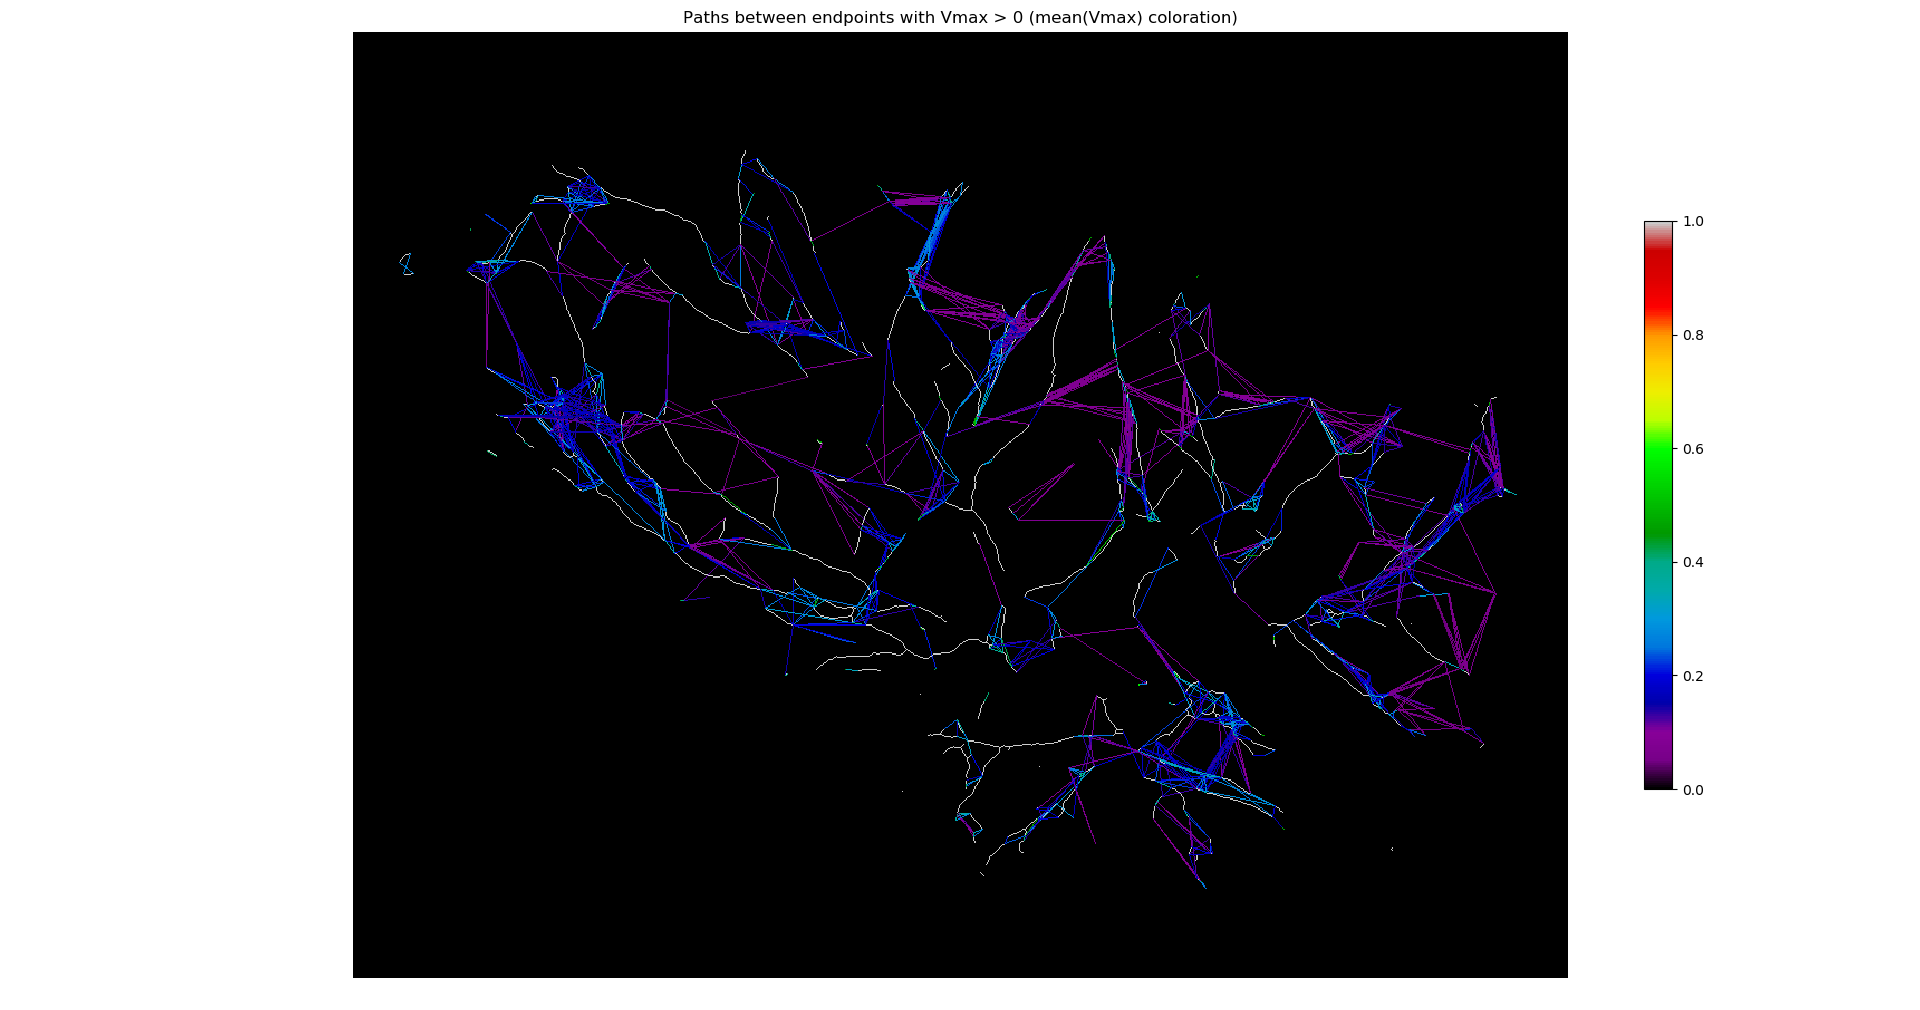
\includegraphics[width=\linewidth]{paths_between_endpoints_positive_score}
  \caption{All lines between endpoints with nonzero $\Vmax$}
  \label{fig:network-completion-all-pairs}
\end{figure}

\begin{figure}
	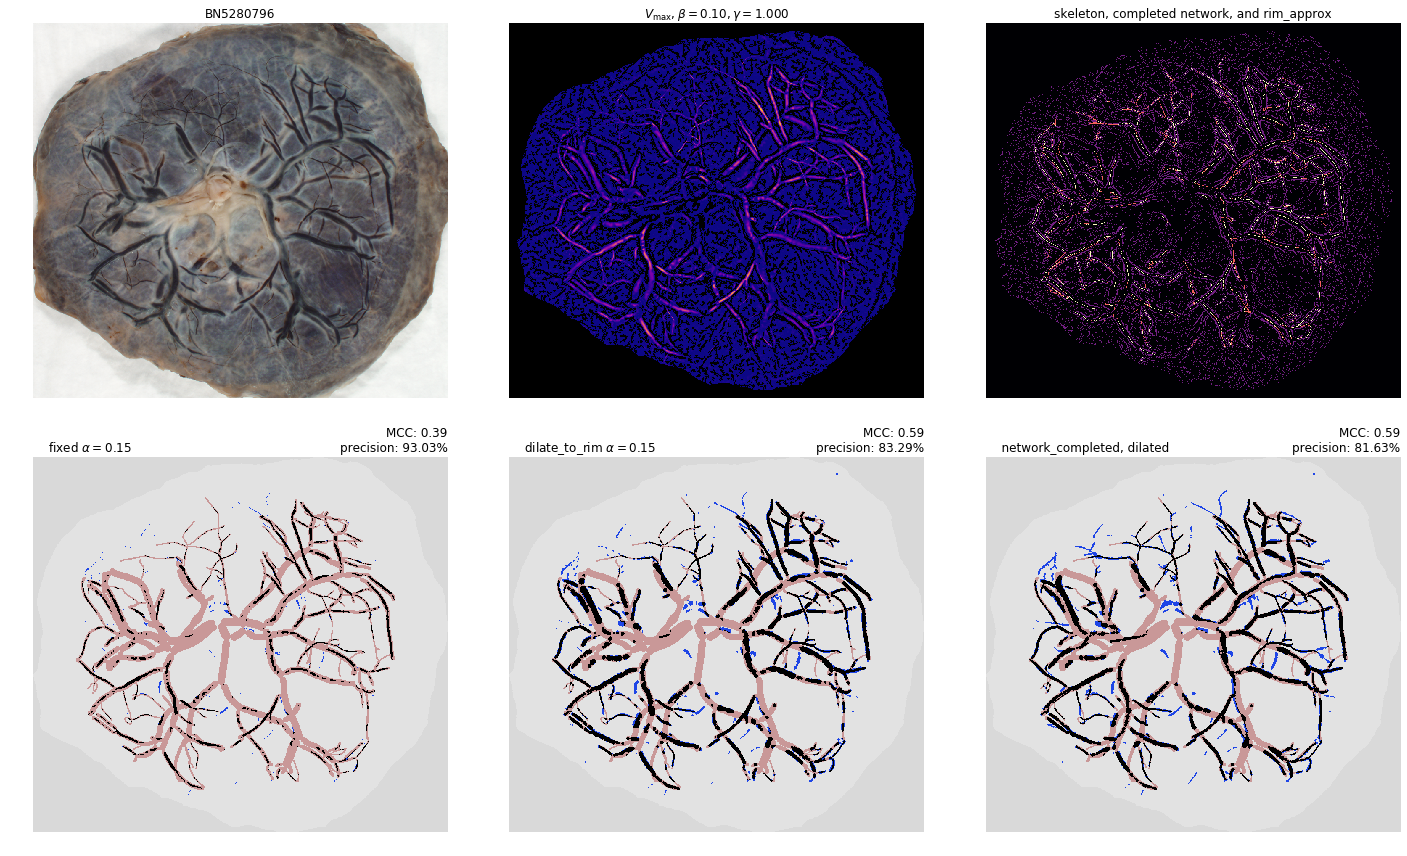
\includegraphics[width=\linewidth]{sample_network_completion}
	\caption{Trough Dilation and Network Completion (Example 1)}
	\label{fig:network-completion-demo-1}
\end{figure}

Finally, we would like to show the efficacy of this method by applying it to more image domains.